% 5_solucion.tex

% Una descripción de la solución propuesta, considerando el hardware que propone utilizar
\section{Descripción de la solución propuesta}

Para la conexión punto a punto que se debe desarrollar, se tienen dos nodos inalámbricos con responsabilidades definidas: un transmisor y un receptor.

Por un lado, el nodo transmisor captura un mensaje de voz, lo digitaliza, lo almacena temporalmente, lo fragmenta en paquetes y lo envía mediante un enlace de radiofrecuencia a \SI{2.4}{\giga\hertz}.
Por otro lado, el nodo receptor permanece en estado de espera activa, detecta el inicio de una transmisión de forma autónoma, recibe los paquetes, reconstruye el archivo de audio y lo reproduce.
A continuación se describe el hardware planteado, algunos parámetros de digitalización seleccionados y el software propuesto.

\subsection{Hardware de cada nodo}

Ahora bien, en esta sección se describe el planteamiento del hardware a utilizar para la realización del proyecto.
Se incluyen los componentes para cada etapa de la transmisión y recepción inalámbrica de audio.

\subsubsection{Raspberry Pi Zero}

La Raspberry Pi Zero se plantea como la unidad de procesamiento principal de cada nodo.
Esta plataforma ejecuta un sistema operativo Linux, lo que permite utilizar herramientas y bibliotecas estándar para la captura y reproducción de audio, el control del módulo de radiofrecuencia y la gestión de los periféricos de entrada y salida.
Al tratarse de un único microprocesador por dispositivo, todas las tareas del sistema, la fragmentación en paquetes, el control del enlace inalámbrico y la señalización de estado, deben ejecutarse sobre esta misma unidad.

Como consideraciones importantes a tomar en cuenta, el sistema operativo se almacena en una tarjeta microSD, según \cite{adafruit_pizero}, que actúa como medio de almacenamiento del sistema y cuya capacidad debe ser suficiente para alojar el sistema operativo, las bibliotecas necesarias y los archivos de audio temporales generados durante la operación.
Además, la configuración inicial del sistema, incluyendo la habilitación del bus SPI y la activación de la interfaz I2S mediante los parámetros y \textit{device-tree overlays} correspondientes, se realiza mediante edición directa del archivo \texttt{config.txt} en la partición de arranque de la tarjeta microSD \cite{adafruit_pizero}.

Respecto a las conexiones disponibles, la Raspberry Pi Zero expone un conector GPIO de $40$ pines que incluye buses SPI, I2C y pines de propósito general, los cuales permiten la conexión de todos los periféricos del sistema (ver Figura \ref{fig:gpio_pinout}) \cite{rpi_hardware}.
Finalmente, algunas variantes de la Pi Zero incluyen módulos WiFi y Bluetooth integrados que no se utilizarán en el proyecto y que podrán deshabilitarse en el sistema operativo para asegurar que la comunicación inalámbrica se realice exclusivamente mediante el enlace de radiofrecuencia en la banda ISM de \SI{2.4}{\giga\hertz}.

\begin{figure}[htb]
    \centering
    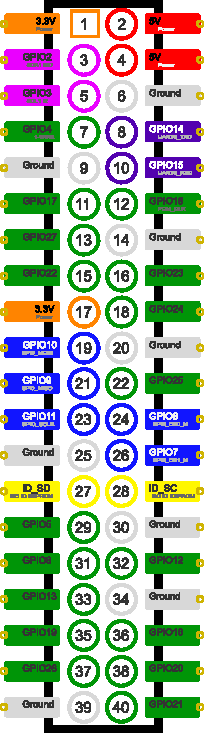
\includegraphics[width=0.25\linewidth]{images/gpio_pinout.pdf}
    \caption{I/O disponible para la Raspberry Pi Zero \cite{tomludlow2021gpio}.}
    \label{fig:gpio_pinout}
\end{figure}

\subsubsection{Transceiver NRF24L01+PA+LNA}

El módulo NRF24L01+PA+LNA es el componente encargado de la comunicación inalámbrica en ambos nodos.
Opera en la banda ISM de \SI{2.4}{\giga\hertz}, que es una banda no licenciada, según las restricciones del proyecto.

A diferencia de la versión básica del NRF24L01, esta variante incorpora un amplificador de potencia (PA) y un amplificador de bajo ruido (LNA), lo que extiende el alcance del módulo y mejora la sensibilidad del receptor respecto a la versión normal.
El PA amplifica la señal transmitida para mayor alcance, mientras que el LNA amplifica las señales recibidas débiles sin introducir ruido significativo.
Estas características son importantes para cumplir los requisitos de distancia del proyecto, tanto los \SI{30}{\meter} del desempeño mínimo como los \SI{100}{\meter} del desempeño óptimo.

El módulo se comunica con la Raspberry Pi Zero mediante el bus SPI \cite{nordic}, lo que simplifica su integración con el sistema operativo Linux a través de bibliotecas disponibles como \texttt{pyRF24} (que se explica posteriormente).
Su tasa de datos configurable de \SI{250}{kbps}, \SI{1}{Mbps} o \SI{2}{Mbps} permite implementar un enlace compatible con distintas tasas de datos requeridas, según la codificación.
Sin embargo, estas corresponden a tasas nominales; la tasa efectiva será inferior debido a encabezados, confirmaciones de recepción, retransmisiones y tiempos de procesamiento en la Raspberry Pi Zero.
Una menor tasa de datos mejora la sensibilidad del receptor y, por lo tanto, permite operar a mayor distancia.
A \SI{1}{Mbps} el módulo ocupa \SI{1}{MHz} de ancho de banda y a \SI{2}{Mbps} ocupa \SI{2}{MHz} \cite{nordic}.
Dado que esta banda es compartida con tecnologías como WiFi y Bluetooth, pueden surgir interferencias durante las pruebas.

El módulo cuenta con $3$ modos de operación: espera (\textit{standby}), transmisor y receptor.
A continuación se explican brevemente:
\begin{enumerate}
    \item Modo espera: en este modo se minimiza la corriente promedio de consumo.
    \item Modo receptor: en este modo el receptor demodula la señal en el canal de radiofrecuencia y presenta los datos demodulados al motor del protocolo de banda base, el cual busca constantemente un paquete válido.
    \item Modo transmisor: al operar como transmisor, el módulo permanece en este estado hasta haber transmitido el último paquete.
\end{enumerate}

Una limitación importante del módulo es que el tamaño máximo del campo de \textit{payload} por paquete es de $32$ bytes, lo que implica que el audio debe fragmentarse en múltiples paquetes y reensamblarse en el receptor \cite{nordic}.
Para un mensaje de \SI{15}{\second} con codificación PCM de \SI{8}{bit} a \SI{8}{\kilo\hertz}, esto equivale a un mínimo de $3750$ paquetes (si todo el \textit{payload} se destinara únicamente a datos de audio).
En la implementación real, la cantidad de paquetes será mayor posiblemente.

El módulo incluye el mecanismo \textit{Enhanced ShockBurst}, el cual incorpora funciones de verificación y confirmación de paquetes a nivel de enlace \cite{nordic}.
Estas características permiten mejorar la confiabilidad de la comunicación inalámbrica sin requerir que todos los mecanismos de recuperación sean implementados desde cero en la aplicación.

La configuración específica del enlace, incluyendo la tasa de transmisión, el tamaño de carga útil, las confirmaciones automáticas y la estrategia de organización de los datos de audio, se detallará posteriormente en la sección correspondiente al protocolo de transmisión.

El módulo permite programar la potencia de transmisión mediante el registro \texttt{RF\_PWR} (por SPI), que ofrece $4$ niveles \cite{nordic}.
Un nivel mayor aumenta el alcance del enlace a costa de un mayor consumo energético.
Cabe señalar que la variante +PA+LNA incorpora un amplificador de potencia externo que eleva la potencia efectivamente radiada y un amplificador de bajo ruido que mejora la sensibilidad en recepción, de modo que los niveles reales del módulo son superiores.

Finalmente, dado que el módulo opera a \SI{3.3}{\volt} y la variante PA LNA puede generar picos de corriente durante la transmisión, el fabricante recomienda alimentarlo mediante un regulador de tensión y/o agregar un capacitor de desacople (de aproximadamente \SI{10}{\micro\farad}) cerca de los pines de alimentación \cite{nordic}, que corresponde al planteamiento realizado.
Este capacitor absorbe los transitorios de corriente durante la transmisión y estabiliza la tensión de alimentación, lo que mejora la confiabilidad del enlace \cite{nordic}.

La Tabla \ref{tab:nrf_pines} describe los pines del módulo y su conexión con la Raspberry Pi Zero.

\begin{table}[htb]
    \centering
    \caption{Asignación de pines para el módulo NRF24L01+PA+LNA en la Raspberry Pi Zero \cite{nordic}.}
    \label{tab:nrf_pines}
    \begin{tabular}{@{}llp{4.5cm}l@{}}
        \toprule
        Pin & Nombre & Función & GPIO \\
        \midrule
        \texttt{VCC}  & Alimentación & Tensión de operación                & \SI{3.3}{\volt}  \\
        \texttt{GND}  & Tierra       & Referencia de tierra                & \texttt{GND} \\
        \texttt{CE}   & Chip Enable  & Activa el módulo en modo TX o RX    & \texttt{GPIO25} \\
        \texttt{CSN}  & Chip Select  & Selección del \textit{slave} SPI    & \texttt{GPIO8} \\
        \texttt{SCK}  & Serial Clock & Señal de reloj del SPI              & \texttt{GPIO11} \\
        \texttt{MOSI} & Master Out   & Datos hacia el módulo               & \texttt{GPIO10} \\
        \texttt{MISO} & Master In    & Datos desde el módulo               & \texttt{GPIO9} \\
        \texttt{IRQ}  & Interrupción & Notifica eventos al microprocesador & N/A \\
        \bottomrule
    \end{tabular}
\end{table}

\begin{figure}[htb]
    \centering
    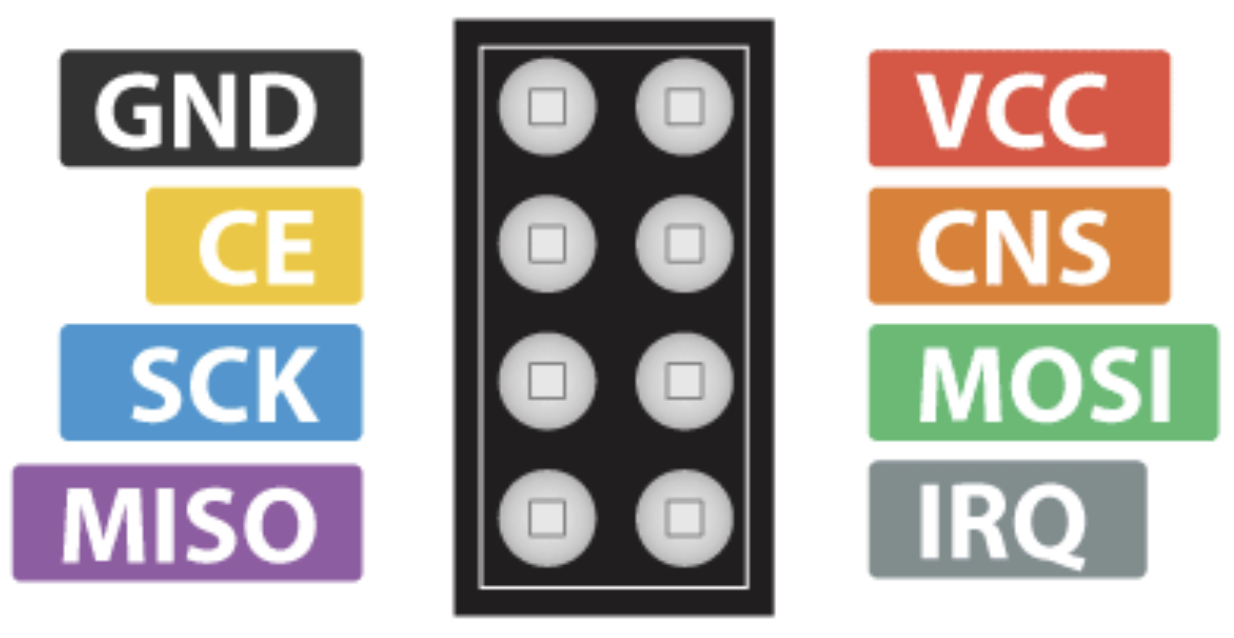
\includegraphics[width=0.35\linewidth]{images/nrf_pinout}
    \caption{Pines del módulo NRF24L01+PA+LNA \cite{nedelkovski2022nrf24l01}.}
    \label{fig:nrf_pinout}
\end{figure}

\subsubsection{Micrófono INMP441}

El micrófono INMP441 es un módulo de salida digital, utilizado en el nodo transmisor para la captura de audio.
A diferencia de los micrófonos analógicos convencionales, el INMP441 integra en un único componente el sensor MEMS, el acondicionamiento de señal, el ADC y los filtros \textit{anti-aliasing}.
Por lo que, entrega datos de audio en formato I2S de $24$ bits \cite{inmp441_datasheet}.
Esto elimina el requerimiento de un convertidor ADC externo y evita los problemas de ruido relacionados con señales analógicas.

Respecto a la alimentación, el módulo opera con una tensión de \SI{1.8}{\volt} y \SI{3.3}{\volt}, lo que lo hace compatible con los pines de \SI{3.3}{\volt} de la Raspberry Pi Zero \cite{inmp441_datasheet}.
Además, su respuesta en frecuencia cubre entre \SI{60}{\hertz} y \SI{15}{\kilo\hertz}, entonces sí contempla el rango de la voz humana entre \SI{300}{\hertz} y \SI{3400}{\hertz} \cite{inmp441_datasheet, tanenbaum2011}.

El módulo incluye además un pin L/R que determina si los datos se transmiten en el canal izquierdo o derecho del \textit{frame} I2S estéreo; al conectarlo a \texttt{GND}, el módulo opera en canal izquierdo, lo que permite su uso en modo mono \cite{inmp441_datasheet}.

Además, una consideración importante es que el INMP441 entrega muestras de $24$ bits, mientras que los esquemas de codificación de audio seleccionados para este proyecto operan con $8$ bits por muestra.
Por esta razón, es necesario aplicar una etapa de conversión de resolución después de la captura, mediante software.
Adicionalmente, el fabricante recomienda conectar un capacitor de desacople de \SI{0.1}{\micro\farad} entre el pin \texttt{VDD} y \texttt{GND} para estabilizar la alimentación del módulo \cite{inmp441_datasheet}.

Finalmente, en la Tabla \ref{tab:inmp441_pines} se describe los pines del módulo y su conexión con la Raspberry Pi Zero; en la Figura \ref{fig:microphone_pinout} se muestran los pines visualmente.

\begin{table}[htb]
    \centering
    \caption{Asignación de pines para el módulo INMP441 en la Raspberry Pi Zero \cite{inmp441_datasheet}.}
    \label{tab:inmp441_pines}
    \begin{tabular}{@{}clp{4.5cm}l@{}}
        \toprule
        Pin  & Nombre & Función & GPIO \\
        \midrule
        \texttt{VDD}  & Alimentación       & Tensión de operación      & \SI{3.3}{\volt} \\
        \texttt{GND}  & Tierra             & Referencia de tierra      & \texttt{GND} \\
        \texttt{SCK}  & Serial Clock       & Señal de reloj I2S        & \texttt{GPIO18} \\
        \texttt{WS}   & Word Select        & Indicador de canal        & \texttt{GPIO19} \\
        \texttt{SD}   & Serial Data        & Datos de audio digitales  & \texttt{GPIO20} \\
        \texttt{L/R}  & Left/Right Select  & Selección de canal        & \texttt{GND} \\
        \bottomrule
    \end{tabular}
\end{table}

\begin{figure}[htb]
    \centering
    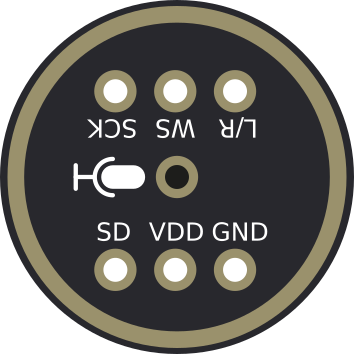
\includegraphics[width=0.35\linewidth]{images/microphone_pinout.png}
    \caption{Pines del micrófono INMP441 \cite{cirkitdesigner_inmp441}.}
  \label{fig:microphone_pinout}
\end{figure}

\subsubsection{Módulo de audio NS4168 con parlante 3070}

Este fue el módulo de audio inicialmente planteado en la propuesta pero no fue utilizado; en su lugar de utilizó el PCM5102 (ver sección \ref{sss:pcm5102}).
Este fue pensado para ser utilizado en el nodo receptor pues agrupa un amplificador NS4168 y un parlante rectangular de $\SI{30}{\milli\meter} \times \SI{70}{\milli\meter}$, lo que simplifica el diseño del hardware al eliminar la necesidad de conectar ambos componentes por separado.

El NS4168 es un amplificador de audio mono con entrada digital I2S y un DAC integrado, lo que le permite recibir la señal de audio en formato I2S desde la Raspberry Pi Zero sin requerir componentes externos \cite{ns4168_datasheet}.
Su potencia de salida máxima es de \SI{2.5}{\watt} con una carga de \SI{4}{\ohm} a \SI{5}{\volt}; esto es suficiente para la reproducción de voz en las condiciones de demostración del proyecto \cite{ns4168_datasheet}.

Asimismo, el NS4168 presenta una función de anti-distorsión (NCN), que detecta automáticamente el recorte de la señal de salida y ajusta la ganancia del amplificador para evitar distorsión audible \cite{ns4168_datasheet}.
También, el módulo incluye un filtro paso-alto que atenúa las frecuencias muy bajas, lo que protege el parlante de señales fuera de su rango de reproducción \cite{ns4168_datasheet}.

Respecto a la alimentación, el módulo opera con una tensión de alimentación de \SI{3.0}{\volt} a \SI{5.5}{\volt} y soporta frecuencias de muestreo de \SI{8}{\kilo\hertz} a \SI{96}{\kilo\hertz}, lo que lo hace compatible con los parámetros de audio seleccionados para este proyecto \cite{ns4168_datasheet}.
El parlante integrado 3070 tiene una impedancia de \SI{4}{\ohm} y una potencia nominal de \SI{3}{\watt}.
La Tabla \ref{tab:ns4168_pines} describe los pines del módulo y su conexión con la Raspberry Pi Zero.

\begin{table}[htb]
    \centering
    \caption{Asignación de pines para el módulo NS4168 en la Raspberry Pi Zero \cite{ns4168_datasheet}.}
    \label{tab:ns4168_pines}
    \begin{tabular}{@{}llp{4.5cm}l@{}}
        \toprule
        Pin & Nombre & Función & GPIO \\
        \midrule
        \texttt{G}   & Tierra           & Referencia de tierra                      & \texttt{GND} \\
        \texttt{V}   & Alimentación     & Tensión de operación                      & \SI{5}{\volt} \\
        \texttt{BLC} & Bit Clock        & Señal de reloj                            & \texttt{GPIO18} \\
        \texttt{LRC} & Left/Right Clock & Indicador de canal del \textit{frame} I2S & \texttt{GPIO19} \\
        \texttt{DIN} & Data In          & Datos de audio digital                    & \texttt{GPIO21} \\
        \bottomrule
    \end{tabular}
\end{table}

\subsubsection{Convertidor digital-analógico PCM5102} \label{sss:pcm5102}

El PCM5102 es un módulo convertidor digital-analógico (DAC), utilizado en el nodo receptor para reconstruir la señal de audio digital recibida mediante el enlace de radiofrecuencia y convertirla en una señal analógica apta para su reproducción.
A diferencia de módulos que integran simultáneamente el convertidor digital-analógico y la etapa de amplificación de potencia, el PCM5102 se encarga únicamente de la conversión de la señal, por lo que requiere un dispositivo de salida externo para reproducir el audio.
El módulo incorpora un conector tipo \textit{jack} de \SI{3.5}{\milli\meter}, al cual se conectó un parlante.
En caso de utilizar un parlante estéreo, reproduce audio en el izquierdo.

Respecto a la alimentación, el módulo opera con una tensión de \SI{5}{\volt} para su etapa principal y utiliza niveles lógicos compatibles con \SI{3.3}{\volt}, lo que permite conectarlo directamente a los pines GPIO de la Raspberry Pi Zero \cite{pcm5102_datasheet}.
Además, soporta frecuencias de muestreo comprendidas entre \SI{8}{\kilo\hertz} y \SI{384}{\kilo\hertz}, con una resolución de hasta $32$ bits por muestra, lo cual supera ampliamente los requerimientos de la configuración de audio seleccionada para este proyecto, correspondiente a audio mono de \SI{8}{\kilo\hertz} y $8$ bits por muestra.

El PCM5102 recibe los datos de audio mediante la interfaz I2S, utilizando las señales \textit{Bit Clock} (\texttt{BCK}), \textit{Left/Right Clock} (\texttt{LRCK}) y \textit{Data In} (\texttt{DIN}).
En la implementación realizada, el pin \texttt{XSMT} se conectó a \SI{3.3}{\volt} para mantener habilitado el convertidor, mientras que los pines \texttt{FMT} y \texttt{DEMP} se conectaron a \texttt{GND} para seleccionar el formato I2S estándar.
Esta configuración permite una integración directa con la Raspberry Pi Zero sin requerir circuitería adicional para el procesamiento del audio digital.

Además, una consideración importante es que el pin \texttt{SCK} no fue utilizado durante la implementación.
Esto se debe a que el PCM5102 incorpora internamente un circuito \textit{Phase-Locked Loop} (PLL), el cual genera automáticamente el reloj interno a partir de las señales I2S recibidas, entonces se elimina la necesidad de suministrar esta señal \cite{pcm5102_datasheet}.

Finalmente, en la Tabla \ref{tab:pcm5102_pines} se describe la asignación de pines del módulo y su conexión con la Raspberry Pi Zero; en la Figura \ref{fig:pcm5102_pinout} se muestran los pines visualmente.

\begin{table}[htb]
    \centering
    \caption{Asignación de pines para el módulo PCM5102 en la Raspberry Pi Zero \cite{pcm5102_datasheet}.}
    \label{tab:pcm5102_pines}
    \begin{tabular}{@{}clp{4.5cm}l@{}}
        \toprule
        Pin & Nombre & Función & GPIO \\
        \midrule
        \texttt{VIN}  & Alimentación & Tensión de operación & \SI{5}{\volt} \\
        \texttt{GND}  & Tierra & Referencia de tierra & \texttt{GND} \\
        \texttt{BCK}  & Bit Clock & Señal de reloj I2S & \texttt{GPIO18} \\
        \texttt{LRCK} & Left/Right Clock & Indicador de canal I2S & \texttt{GPIO19} \\
        \texttt{DIN}  & Data In & Datos de audio digitales & \texttt{GPIO21} \\
        \texttt{XSMT} & Soft Mute & Habilitación del convertidor & \SI{3.3}{\volt} \\
        \texttt{FMT}  & Format Select & Selección del formato I2S & \texttt{GND} \\
        \texttt{DEMP} & De-emphasis & Deshabilita el filtro de preénfasis & \texttt{GND} \\
        \texttt{SCK}  & System Clock & Reloj maestro externo & Sin conectar \\
        \bottomrule
    \end{tabular}
\end{table}

\begin{figure}[htb]
    \centering
    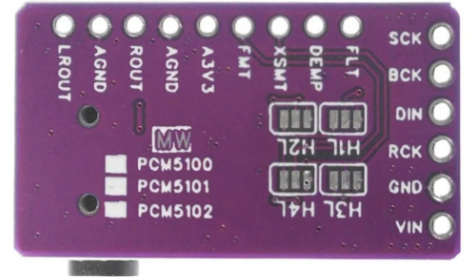
\includegraphics[width=0.42\linewidth]{images/pcm5102_pinout.png}
    \caption{Pines del módulo PCM5102 \cite{SCCCLTD_PCM5102}.}
    \label{fig:pcm5102_pinout}
\end{figure}

\subsubsection{Alimentación}

Ambos nodos deben operar con autonomía energética.
Para la solución se plantea el uso de un \textit{powerbank} como fuente de alimentación.
La Raspberry Pi Zero recibe \SI{5}{\volt} directamente del \textit{powerbank} a través de su puerto microUSB, que es la forma estándar de alimentación de esta plataforma \cite{adafruit_pizero}.

La distribución de tensiones dentro de cada nodo requiere consideración especial debido a que los componentes operan a distintos niveles de tensión.
Para garantizar una tensión estable al módulo de radiofrecuencia, se plantea el uso de uno de los reguladores de tensión disponibles en el laboratorio, configurado para derivar \SI{3.3}{\volt} desde la línea de \SI{5}{\volt} del \textit{powerbank}.
Asimismo, se colocarán capacitores de desacople cerca de los pines de alimentación para reducir caídas transitorias de tensión para algunos de los equipos, según sea necesario (como se comentó individualmente antes).

\subsubsection{Botones y LEDs}

Cada nodo incluye un botón y tres LEDs en cumplimiento con las especificaciones del proyecto, que exigen un interruptor para iniciar la operación y una luz piloto que indique actividad.

El botón se conecta a un pin GPIO de la Raspberry Pi Zero configurado como entrada digital con resistencia de \textit{pull-up} interna, de forma que al presionarlo se genera una transición de nivel alto a nivel bajo que el software detecta como evento de inicio.
En el nodo transmisor, la presión del botón da inicio a la captura del audio.

Los tres LEDs se conectan cada uno a un pin GPIO configurado como salida digital, en serie con una resistencia limitadora de corriente eléctrica para proteger tanto el LED como el pin GPIO.
El esquema de señalización planteado utiliza un LED verde, uno amarillo y uno rojo, que reflejan la etapa de operación en curso (esto se explica más adelante en detalle).

En la Tabla \ref{tab:gpio_botones_leds} se resumen las conexiones para estos componentes en la Raspberry Pi Zero.

\begin{table}[htb]
    \centering
    \caption{Asignación de pines GPIO para los botones y LEDs en la Raspberry Pi Zero.}
    \label{tab:gpio_botones_leds}
    \begin{tabular}{@{}lp{4.5cm}l@{}}
        \toprule
        Componente   & Función & GPIO \\
        \midrule
        Botón        & Inicio de captura (transmisor)                   & \texttt{GPIO17} \\
        LED verde    & Indica estado listo / transmisión exitosa        & \texttt{GPIO27} \\
        LED amarillo & Indica proceso en curso                          & \texttt{GPIO22} \\
        LED rojo     & Indica error                                     & \texttt{GPIO23} \\
        \bottomrule
    \end{tabular}
\end{table}

\subsubsection{Diagrama de hardware}

Después de haber detallado las características de cada uno de los componentes contemplados para el desarrollo del proyecto, se realizaron dos diagramas de hardware de la arquitectura del sistema: uno para el nodo transmisor y otro para el nodo receptor.
Estos se muestran en las Figuras \ref{fig:diagrama_transmisor} y \ref{fig:diagrama_receptor}.

\begin{figure}[htb]
    \centering

    \begin{subfigure}{0.75\columnwidth}
        \centering
        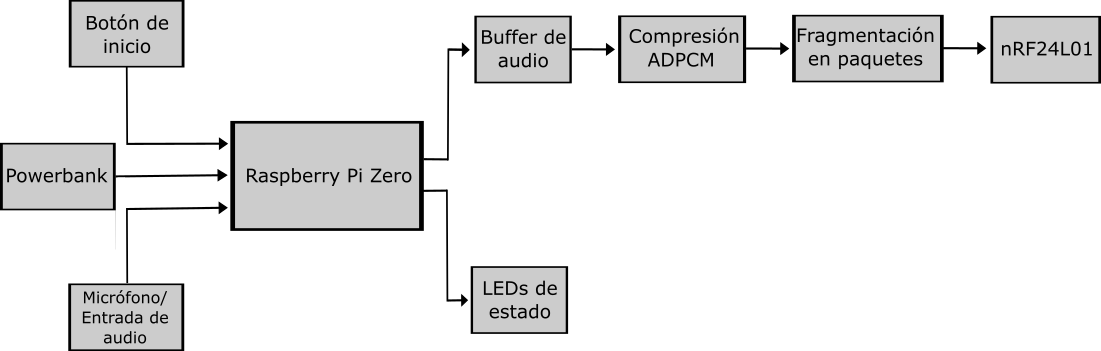
\includegraphics[width=\columnwidth]{images/diagrama_emisor.png}
        \caption{Diagrama de bloques del transmisor.}
        \label{fig:diagrama_transmisor}
    \end{subfigure}

    \vspace{1em}

    \begin{subfigure}{0.75\columnwidth}
        \centering
        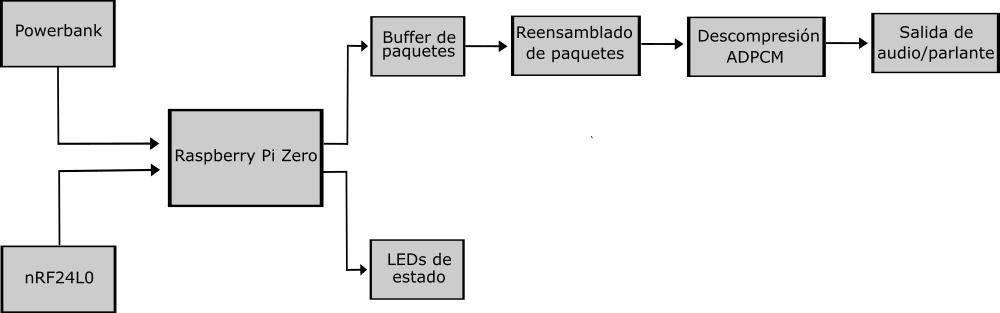
\includegraphics[width=\columnwidth]{images/diagrama_receptor.png}
        \caption{Diagrama de bloques del receptor.}
        \label{fig:diagrama_receptor}
    \end{subfigure}

    \caption{Diagramas de bloques del sistema de comunicación.}
    \label{fig:diagramas}
\end{figure}

\subsection{Parámetros de digitalización seleccionados}

Antes se comentaron los aspectos de hardware necesarios para la solución del proyecto, ahora se explicarán algunos detalles relacionados con el almacenamiento, transmisión y recepción de la señal de audio.

A partir del análisis de esquemas de codificación de audio presentado en el avance anterior, se selecciona como configuración base una frecuencia de muestreo de \SI{8}{\kilo\hertz}, una resolución de $8$ bits por muestra y un canal mono.
Esta configuración produce una tasa de bits de \SI{64}{kbps} y archivos de aproximadamente \SI{40}{kB}, \SI{80}{kB} y \SI{120}{kB} para mensajes de $5$, $10$ y $15$ segundos, respectivamente.
Con lo anterior, resulta en un mínimo de $1250$, $2500$ y $3750$ paquetes de $32$ bytes para cada caso (si todo el \textit{payload} se destinara a datos de audio).
En la implementación real, el número de paquetes será mayor debido a los campos de control requeridos por la estructura de la transferencia.

El formato de transmisión es PCM crudo, que minimiza el \textit{overhead} de formato y el encabezado WAV se reconstruye en el receptor a partir de los parámetros conocidos del sistema.
Como optimización sobre esta base, se implementó la compresión ADPCM, que reduce la tasa de bits a aproximadamente \SI{32}{kbps} y el número de paquetes a una fracción del original, dentro del alcance del desempeño óptimo del proyecto.
El códec es seleccionable mediante configuración (PCM o ADPCM) y se emplea ADPCM de forma predeterminada; el receptor detecta automáticamente el códec utilizado a partir del paquete \texttt{START}.
La Tabla \ref{tab:params_audio} resume los parámetros seleccionados para la configuración base del sistema.

\begin{table}[htb]
\centering
\caption{Parámetros de digitalización seleccionados para la configuración base.}
\label{tab:params_audio}
\begin{tabular}{@{}lp{5.5cm}@{}}
\toprule
Parámetro & Valor \\
\midrule
Frecuencia de muestreo  & \SI{8}{\kilo\hertz} \\
Resolución              & $8$ bits por muestra \\
Canales                 & Mono \\
\addlinespace
Formato base            & PCM crudo \\
Formato en receptor     & WAV \\
\addlinespace
Tasa de bits            & \SI{64}{kbps} \\
Tamaño \SI{5}{\second}  & \SI{40}{kB} (mínimo $1250$ paquetes) \\
Tamaño \SI{10}{\second} & \SI{80}{kB} (mínimo $2500$ paquetes) \\
Tamaño \SI{15}{\second} & \SI{120}{kB} (mínimo $3750$ paquetes) \\
\addlinespace
Códec (seleccionable)   & PCM / ADPCM \\
\bottomrule
\end{tabular}
\end{table}

\subsection{Software propuesto}

El software de cada nodo se desarrolló en Python sobre el sistema operativo Linux de la Raspberry Pi Zero.
Esta elección permite aprovechar las bibliotecas disponibles para el control de periféricos, la captura y reproducción de audio y la comunicación con el módulo de radiofrecuencia.
En la Tabla \ref{tab:bibliotecas} se resume las bibliotecas seleccionadas para cada función del sistema.

\begin{table}[htb]
    \centering
    \caption{Bibliotecas de software seleccionadas para la implementación.}
    \label{tab:bibliotecas}
    \begin{tabular}{@{}p{3.5cm}lp{4.5cm}@{}}
        \toprule
        Función & Biblioteca & Justificación \\
        \midrule
        Control NRF24L01    & \texttt{pyRF24} \mbox{\cite{nrf24_pyrf24}}   & Wrapper en Python de la biblioteca RF24 \\
        Captura de audio y reproducción & \texttt{sounddevice} \mbox{\cite{spatialaudio_sounddevice}} & Interfaz para captura desde el micrófono I2S y reproducción \\
        Archivo WAV         & \texttt{wave} \mbox{\cite{python_wave}}    & Módulo de Python para construir el encabezado WAV sobre datos PCM \\
        Muestras de audio   & \texttt{numpy} \mbox{\cite{numpy2025}}  & Manipulación de muestras y conversión de $24$ a $8$ bits \\
        GPIO                & \texttt{gpiozero} \mbox{\cite{gpiozero}} & Control de botones y LEDs \\
        \bottomrule
    \end{tabular}
\end{table}

Una consideración importante es la distinción entre el formato de transmisión y el formato de almacenamiento en el receptor.
Durante la transmisión se envían bytes PCM \textit{raw} sin encabezado, lo que minimiza el \textit{overhead} por paquete.
Al finalizar la recepción, el nodo receptor utiliza el módulo \texttt{wave} para construir el encabezado WAV de $44$ bytes a partir de los parámetros conocidos del sistema, con lo que se produce un archivo reproducible.

El control del módulo NRF24L01+PA+LNA se realiza mediante \texttt{pyRF24}, que es el \textit{wrapper} Python de la biblioteca \texttt{RF24}.
Esta biblioteca expone los registros del módulo y permite configurar el canal de radiofrecuencia, la tasa de datos, la potencia de transmisión y los parámetros del mecanismo \textit{Enhanced ShockBurst}.
La fragmentación del audio en paquetes de $32$ bytes, la numeración de secuencia y el reensamblado en el receptor se implementaron de forma manual.